%\documentclass{article}
%\usepackage{graphicx,subfigure}
%\begin{document}

\begin{figure}[h]
  \centering
   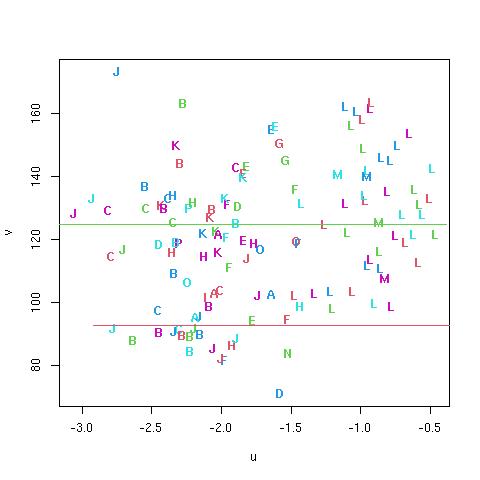
\includegraphics[width=0.9\textwidth]{carter68/hypcoordcarter68.png}
  \caption{Plot of breed means for hyperbolic coordinates $u$ and $v$ for data from Carter(1968)~\cite{cart:68}. Red line shows points with a $k$ value of 8600, green line a $k$ value of 15600.}
  \label{fig:hypcoord}
\end{figure}

%\end{document}

